\documentclass[aspectratio=169]{beamer}
\usetheme[block=fill]{metropolis}
\usepackage{tikz}
\usetikzlibrary{shapes.geometric, arrows.meta, positioning, calc}

\title{Building a Reproducible Scholarly Search Toolkit}
\subtitle{Episode 8: Rate Limiting with Token Buckets}
\author{Scholar Search Kit}
\date{}

\begin{document}

\begin{frame}[plain]
  \titlepage
\end{frame}

\begin{frame}{Episode Goal}
  \begin{alertblock}{The Goal}
    Implement a Token Bucket algorithm to strictly enforce polite API usage across our system.
  \end{alertblock}
  \vspace{0.5cm}
  If we bombard Crossref or Semantic Scholar, they will permanently ban our IP. A simple \texttt{time.sleep()} is too naive for bursting workflows. We need a continuous token bucket.
\end{frame}

\begin{frame}{The Token Bucket Algorithm}
  \begin{center}
  \resizebox{0.7\linewidth}{!}{
  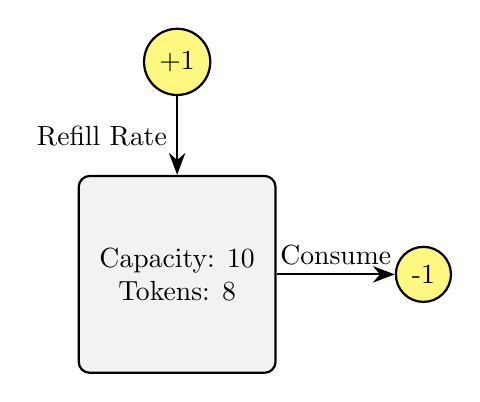
\begin{tikzpicture}[
      node distance=1.5cm and 2cm,
      bucket/.style={rectangle, draw, thick, rounded corners, minimum width=2.5cm, minimum height=2.5cm, align=center, fill=black!5},
      token/.style={circle, draw, thick, minimum size=0.5cm, fill=yellow!50},
      arrow/.style={-{Stealth[scale=1.2]}, thick}
    ]
    
    \node[bucket] (b) {Capacity: 10\\Tokens: 8};
    \node[token, above=1cm of b] (t1) {+1};
    \node[token, right=1.5cm of b] (t2) {-1};
    
    \draw[arrow] (t1) -- node[left] {Refill Rate} (b);
    \draw[arrow] (b) -- node[above] {Consume} (t2);
  \end{tikzpicture}
  }
  \end{center}
  \vspace{0.2cm}
  Tokens refill at a steady rate up to a max capacity. Every API call consumes a token. If zero tokens remain, we block.
\end{frame}

\begin{frame}{Implementation: \texttt{TokenBucket}}
  \begin{block}{State without Threads}
    We can implement this entirely with math and timestamps, avoiding complex thread locking.
  \end{block}
  
  \begin{itemize}
      \item Calculate time elapsed since last check.
      \item Add tokens based on elapsed time $\times$ refill rate.
      \item Cap at max capacity.
      \item If requested tokens $\le$ available, deduct and proceed. Else, sleep.
  \end{itemize}
\end{frame}

\begin{frame}{Why not a Sliding Window?}
  \begin{block}{Simplicity vs Strictness}
    Sliding windows (e.g., max 100 requests per 5 minutes) require tracking a log of every timestamp.
  \end{block}
  
  \begin{itemize}
      \item The Token Bucket uses $O(1)$ memory (just tracking the last timestamp and token count).
      \item It natively allows for initial bursts while enforcing a steady long-term average.
  \end{itemize}
\end{frame}

\begin{frame}{Verification}
  \begin{alertblock}{Success Criteria}
    \begin{itemize}
        \item Consuming tokens depletes the count.
        \item Waiting allows tokens to refill exactly up to the burst limit.
        \item Requesting a token when empty forces a calculated sleep.
    \end{itemize}
  \end{alertblock}
\end{frame}

\end{document}
